\chapter{Methodology and Tools}
\label{chap:Methodology}

\section{Hardware and Software Tools}

Our methodology relies on a combination of software frameworks for machine learning and a target embedded hardware platform. We describe the tools and platforms used below.

\subsection*{TensorFlow and Keras}

We built and trained all neural networks using TensorFlow (version 2.18) with the Keras API. The \texttt{TakuNetModel} class is a Keras \texttt{Model} under the hood, composed of standard Keras layers such as \texttt{Conv2D}, \texttt{DepthwiseConv2D}, and \texttt{Dense}. This choice provided high-level flexibility in defining arbitrary model architectures.

Training was performed on a workstation with GPU support, The GPU used in our experiments was the \textbf{Tesla V100 SXM2 32GB}.
In addition, we used auxiliary Python libraries: \texttt{scikit-learn} for computing evaluation metrics (precision, recall, F1-score), and \texttt{pandas} for logging results. The genetic algorithm are also implemented in Python using \texttt{NumPy} and \texttt{TensorFlow}. This entire experimentation framework runs on DTU's HPC.

\subsection*{Power Profiler Kit II}

The \textbf{Power Profiler Kit II (PPK2)} from Nordic Semiconductor was used to both power the Arduino Nano BLE 33 Sense and measure its current consumption during inference. The PPK2 was operated in source meter mode, supplying a constant voltage while simultaneously recording the current draw over time. This setup enabled reliable and high-resolution profiling of the power usage associated with different model configurations deployed on the device.

The collected current data, combined with the inference time, was used to estimate the total energy consumption for each model. This allowed for a practical evaluation of the trade-offs between model accuracy, size, and energy efficiency ~\cite{nordicPPK2}.

\subsection*{TensorFlow Lite for Microcontrollers}

To enable deployment of models trained on a PC to resource-constrained microcontrollers, we utilized TensorFlow Lite. Specifically, trained models were first converted to the TensorFlow Lite FlatBuffer format and then deployed using TensorFlow Lite for Microcontrollers (TFLite Micro).

TFLite Micro is a highly optimized inference engine tailored for memory-limited embedded systems. It supports only a subset of TensorFlow operations, which guided our model design to include only operators compatible with this runtime.

For the target hardware platform, we selected the \textbf{Arduino Nano 33 BLE Sense}, one of the most widely used microcontrollers for embedded machine learning applications. A detailed description of the deployment procedure, along with the specific constraints of the device, is provided in the \hyperref[chap:DeploymentEnvironment]{relevant chapter}.

\section{System Architecture}

When applying Neural Architecture Search (NAS) to microcontroller deployment, the workflow typically follows a specific pipeline, illustrated in Figure~\ref{fig:architectural_pipeline}.

During each iteration of the NAS process, a candidate neural network model is generated. This model is trained and evaluated on a validation dataset. Then, it is converted into a TensorFlow Lite (\texttt{.tflite}) format and subsequently into a C header file. This conversion is necessary to enable deployment on microcontrollers through environments such as Arduino.

It is important to note that the \texttt{.tflite} version of a model may not behave identically to its original Keras counterpart. This discrepancy is primarily caused by the conversion process, which often includes optimizations such as \textit{quantization}, \textit{operator fusion}, and other \textit{graph transformations} designed to reduce model size and improve inference efficiency on embedded hardware.

Among these, \textbf{quantization} is the most impactful. It involves converting the original 32-bit floating-point weights and activations into lower precision formats such as \texttt{int8} or \texttt{float16}, depending on the chosen quantization scheme. Each format offers different trade-offs:

\begin{itemize}
    \item \textbf{Full Integer Quantization (int8)}: Converts all weights and activations to 8-bit integers. This significantly reduces memory and computational requirements and is supported by most microcontrollers. However, it can introduce approximation errors due to reduced numerical precision.
    
    \item \textbf{Float16 Quantization}: Converts weights to 16-bit floating point values while typically leaving activations in \texttt{float32}. It provides a balance between reduced model size and higher numerical fidelity but requires hardware support for float16 inference.
\end{itemize}

Therefore, it is essential to \textbf{re-evaluate the model’s accuracy after conversion} to confirm that the \texttt{.tflite} version performs similarly to the original model. In practice, when using full integer quantization with a properly selected representative dataset, the accuracy loss is often negligible \cite{tensorflow2023quantization}.

After post-conversion validation, the model is deployed to the microcontroller, where key hardware-related metrics such as \textit{RAM usage}, \textit{Flash memory consumption}, and \textit{energy consumption} are measured. These hardware measurements are incorporated into the model’s overall fitness evaluation, guiding the NAS algorithm toward architectures that are not only accurate but also resource-efficient.

This process is iteratively repeated using an evolutionary algorithm until a predefined time limit is reached. Upon termination, the best models are presented as a \textbf{Pareto front}, representing the trade-off between competing objectives such as predictive accuracy and hardware efficiency.

\begin{figure}[ht]
    \centering
    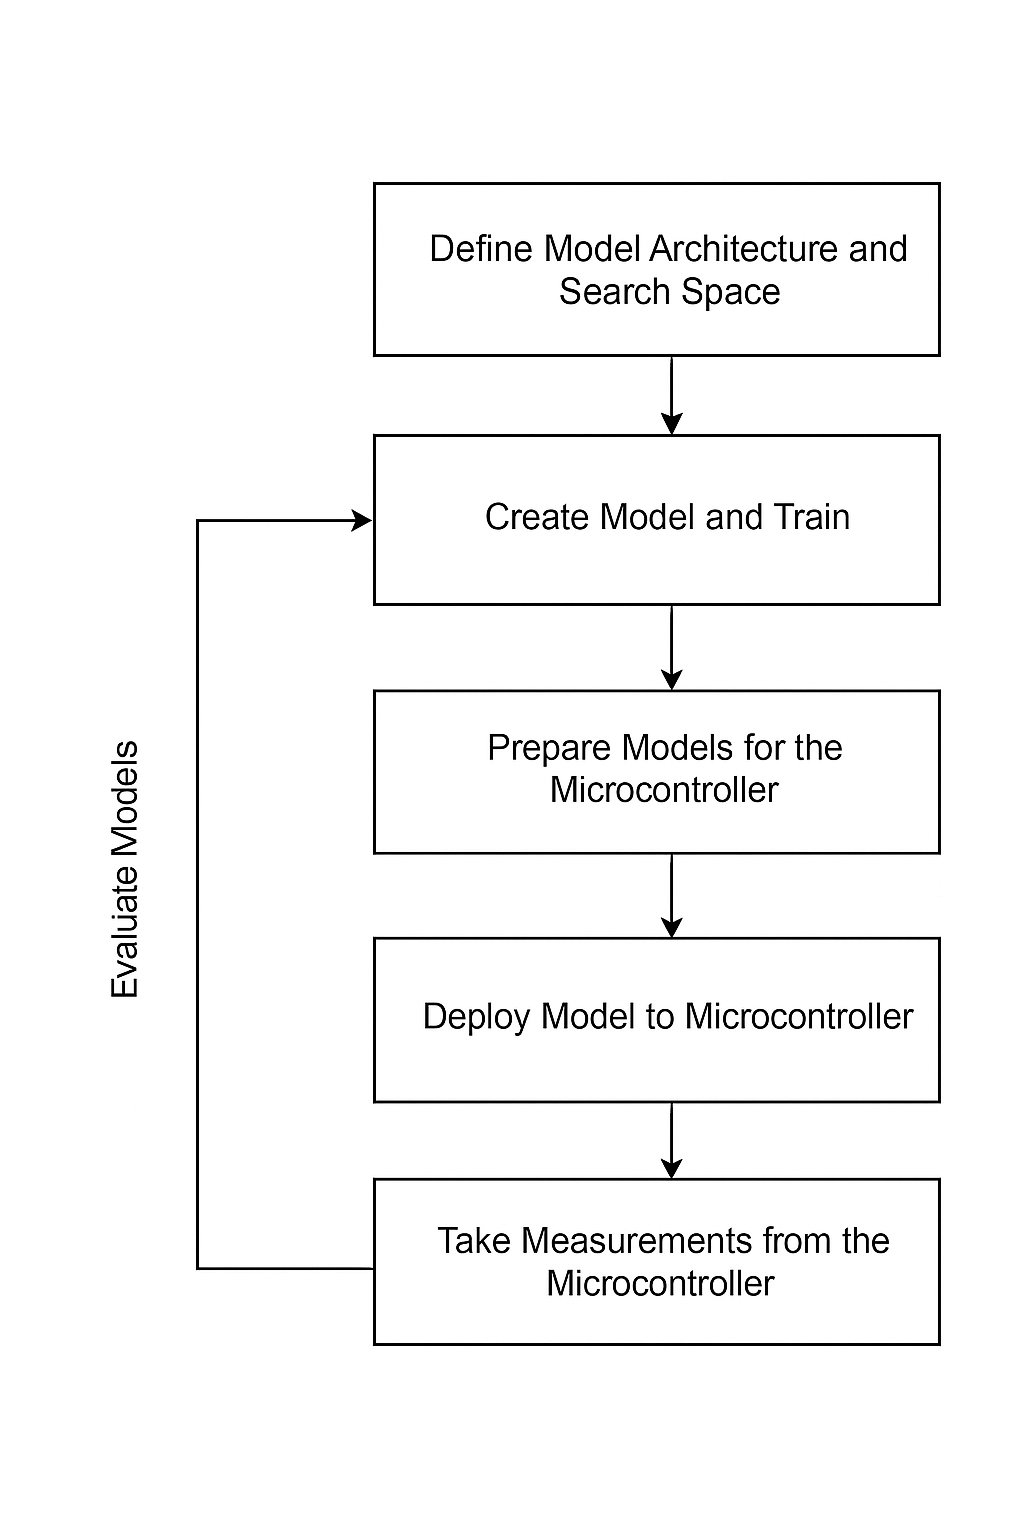
\includegraphics[width=0.6\linewidth]{Pictures/OldMethodology.png}
    \caption{Typical NAS pipeline for deployment on microcontrollers.}
    \label{fig:architectural_pipeline}
\end{figure}



\subsection{Timing of the Processes}

To achieve satisfactory performance, the training process typically requires at least 70 epochs, which takes approximately 20 to 30 minutes, depending on the model architecture and dataset size. The subsequent conversion and quantization steps generally take between \textit{X} and \textit{Y} minutes, taking into consideration the conversion and the procedure to test the accuracy. Model deployment—including compilation, tensor allocation, and inference execution (detailed further in Chapter~\ref{chap:DeploymentEnvironment})—requires approximately 3 minutes. Since the measurement of hardware metrics (such as RAM, Flash, and energy consumption) is integrated into the deployment step, its overhead is considered negligible.

These values provide useful insight into where optimization efforts should be focused. In particular, reducing the time required for training is crucial for increasing the number of models that can be evaluated within a given time frame. This, in turn, enhances the effectiveness of the NAS process by allowing a broader exploration of the search space, thereby increasing the likelihood of discovering high-performing architectures.

To address these limitations, several workflow optimizations were introduced. These are discussed in the following subsection.

\subsection{Optimized Version}
Given the timing constraints outlined above, we adopted several strategies to streamline the NAS process:

\begin{itemize}
    \item \textbf{Training Time Reduction}: We explored techniques to shorten the training phase, including early stopping and training-time proxies.

    \item \textbf{Proxy-Based Evaluation}: To reduce the deployment cost for each model, we developed lightweight proxies to estimate hardware performance (e.g., memory usage or inference latency) without any deployment. These proxies allowed to evaluate and compare models without the additional overhead.
    
    \item \textbf{Development Conversion}: Without the need of deployment each model, we did not have to convert the non-Pareto Front models into .tflite model. This saved the conversion time for the vast majority of models.
    
    \item \textbf{Deployed Model Accuracy}: We incoperate techniques to make the quantization as efficient as possible enabling to trust post-deployment behavior without having to test every version extensively
    
\end{itemize}

A visual summary of the improved workflow is shown in Figure~\ref{fig:workflow_optimization}.


\begin{figure}[ht]
    \centering
    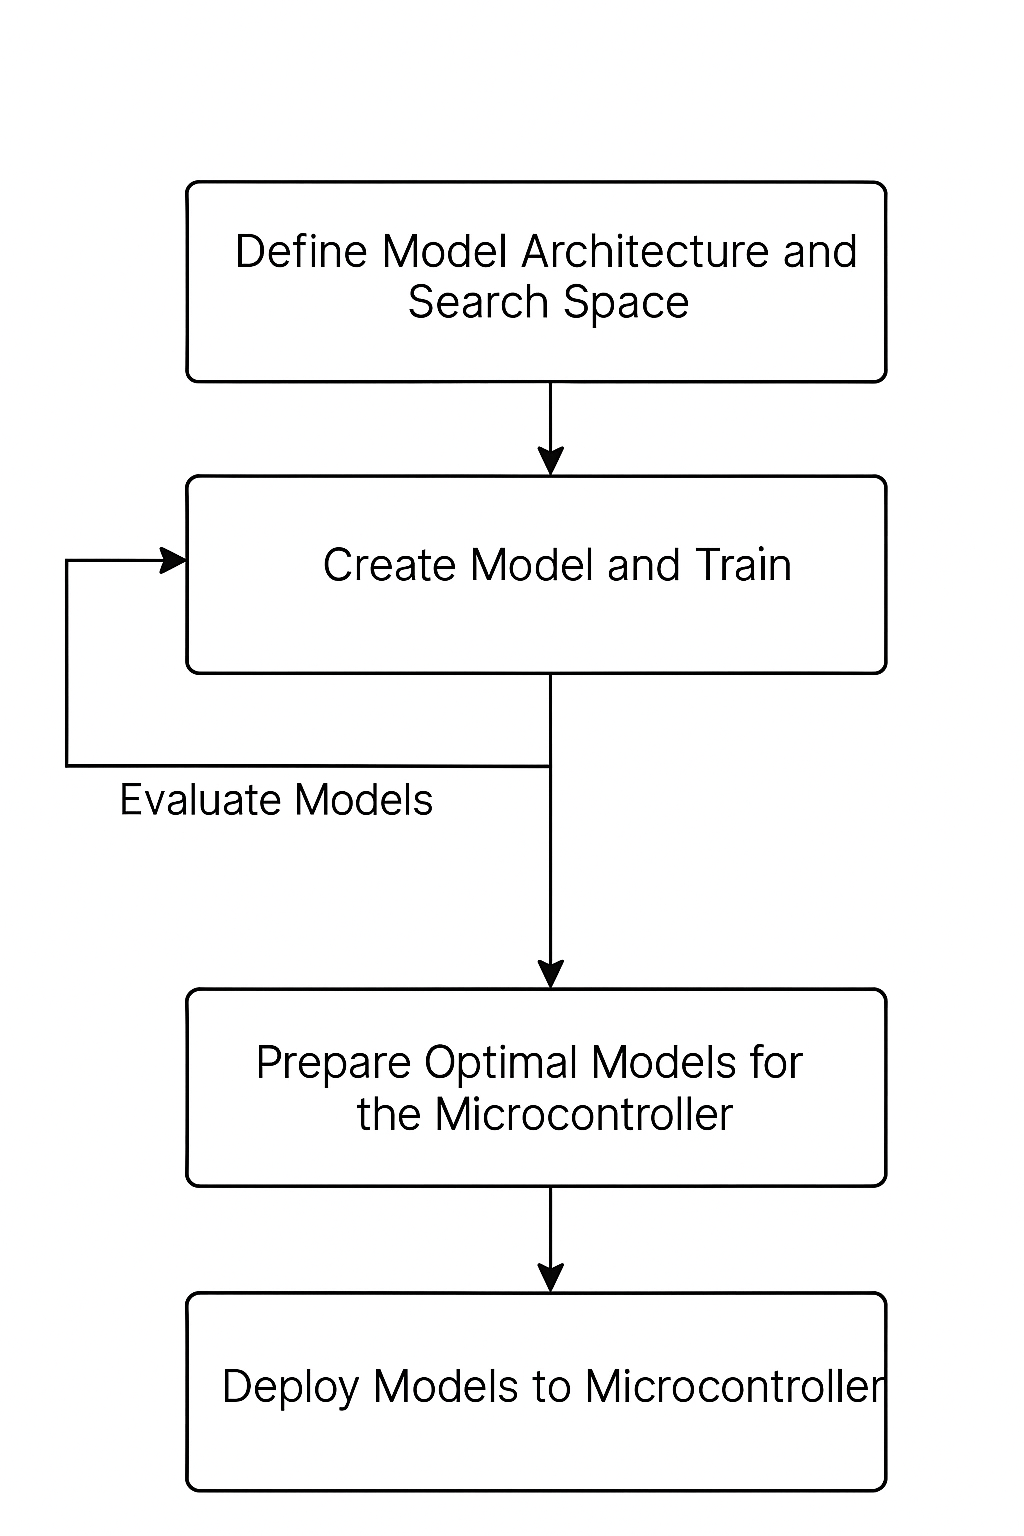
\includegraphics[width=0.6\linewidth]{Pictures/NewMethodology.png}
    \caption{Optimized NAS pipeline for deployment on microcontrollers.}
    \label{fig:workflow_optimization}
\end{figure}



\begin{comment}
The overall system is designed to automatically search for a resource-efficient convolutional neural network (CNN) architecture and deploy it on a microcontroller. Figure~\ref{fig:architectural_pipeline} outlines the methodology pipeline, which consists of the following stages: 

\begin{enumerate}
    \item Defining a flexible model architecture and search space,
    \item Training and evaluating candidate models (including profiling their resource usage),
    \item An evolutionary search loop (Neural Architecture Search) driven by a genetic algorithm with a surrogate model, and
    \item Modify the model accordingly to be eligible to deployed in the microcontroller.
    \item Deploy the model
\end{enumerate}

Each stage is described below and will be explained in specific chapter.


\TODO{Here change the image to be a loop, also add rough timing to show how much time is spent in each stage}
\begin{figure}[H]
    \centering
    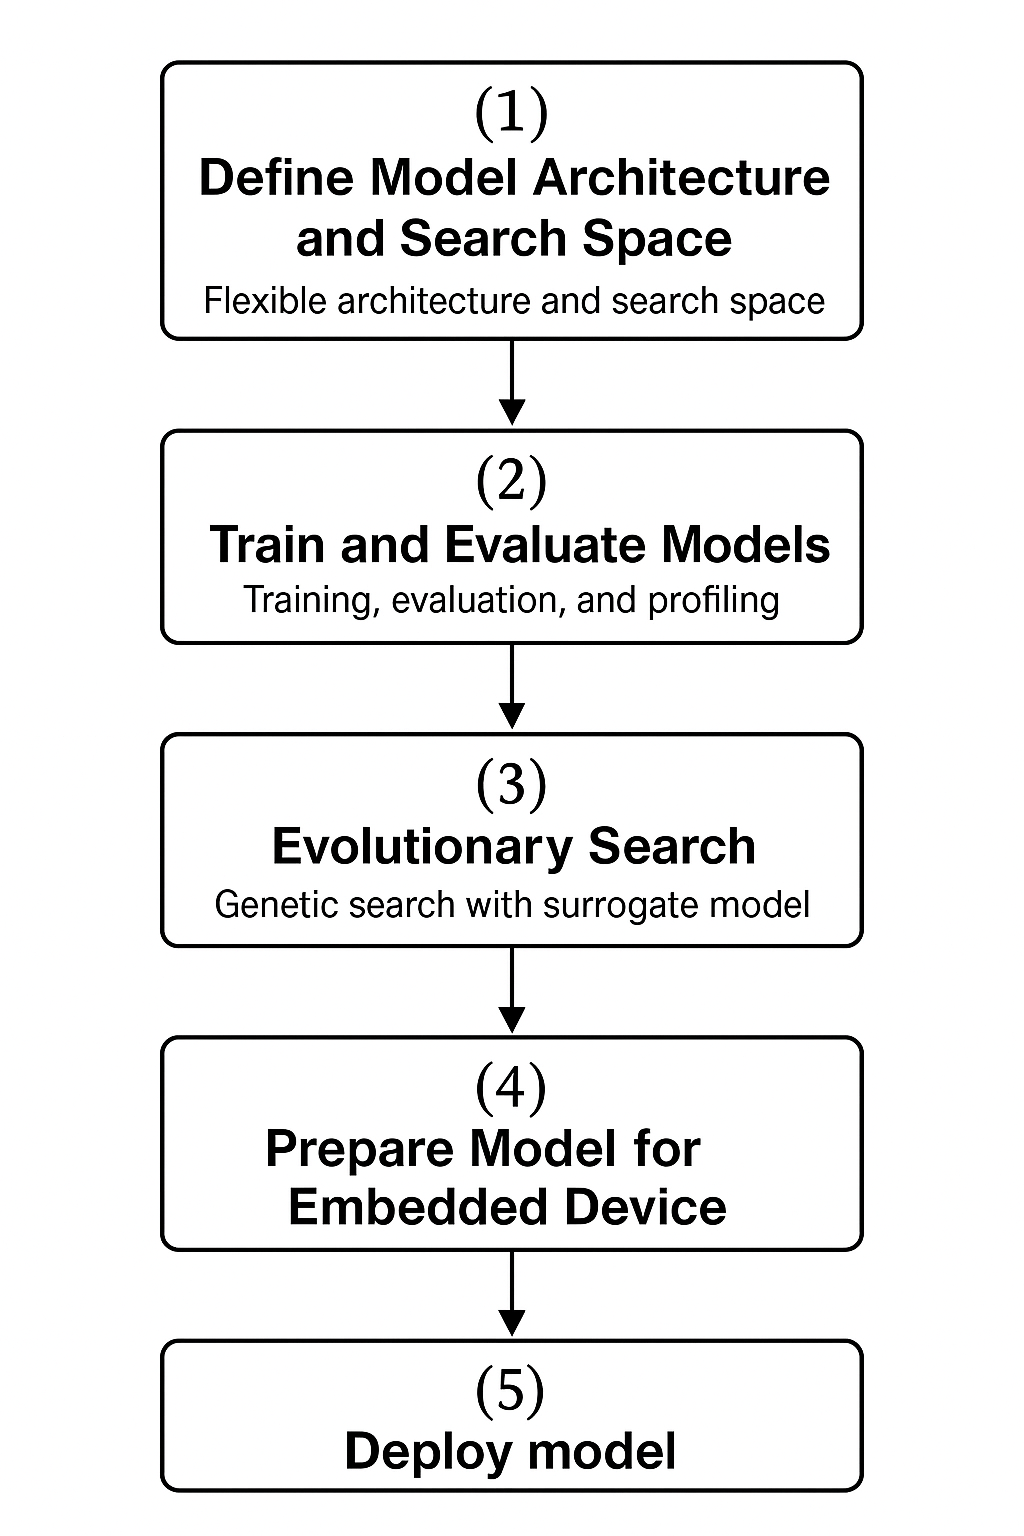
\includegraphics[width=0.6\linewidth]{Pictures/Architecture.png}
    \caption{Architectural pipeline}
    \label{fig:architectural_pipeline}
\end{figure}
    
\end{comment}









\subsection{Define Model Architecture and Search Space}

We developed a custom model class, \texttt{TakuNetModel}, capable of constructing convolutional neural networks (CNNs) based on a set of architectural parameters. These parameters, sampled from a predefined search space, determine the network's configuration, such as the number of layers, kernel sizes, and other key design choices. The model is assembled in a modular fashion: an initial stem block processes the input, followed by a sequence of repeated stage blocks, and concluding with a refiner block that generates the final classification output. A detailed explanation of each layer is provided in \hyperref[chap:Architecture]{Chapter 5}.

All configurable parameters that define the architecture are stored in a \texttt{.json} file, which represents the \textbf{search space} for our algorithm.



\subsection{Training and Evaluation models}

The training and evaluation phase is a critical part of the overall pipeline, responsible for assessing the performance and efficiency of each candidate CNN architecture generated during the Neural Architecture Search (NAS) process. The primary goal is to determine how well each model performs not only in terms of classification accuracy, but also in terms of its resource consumption, making it suitable for deployment on resource-constrained microcontrollers.

\begin{enumerate}

    \item \textbf{Dataset CIFAR-100}
    
    All models are trained and evaluated using the CIFAR-100 dataset which consists of:
\begin{itemize}
    \item 60,000 color images of size 32x32 pixels
    \item 100 distinct classes (600 images per class)
\item a standard split: 50,000 training images and 10,000 test images

\end{itemize}

The dataset is challenging due to its high number of classes, which increases the importance of using evaluation metrics beyond just accuracy.

    \item \textbf{Model Training}
    Each candidate's architecture is trained from scratch using TensorFlow 2.18.0, with GPU acceleration enabled where available. The training pipeline includes the following steps:
    
\begin{itemize}
    \item \textbf{Initialization:} Models are initialized and built dynamically based on sampled architecture parameters from the search space.
    \item \textbf{Training Metrics:} \textit{Training Accuracy} is recorded per epoch to monitor learning progress and \textit{Validation Accuracy} is used to estimate generalization and prevent overfitting.

\end{itemize}

Training is kept consistent across models to ensure fair comparison in the NAS loop.
\item \textbf{Post-Training Evaluation}

After training, each model is evaluated on the test set using several key performance metrics: 
\begin{itemize}
    \item \textbf{Test Accuracy}: Overall classification accuracy across all test images.
    \item \textbf{Precision}: The proportion of correct positive predictions per class.
    \item \textbf{Recall}: The proportion of actual positives that were correctly identified.
\end{itemize}

These metrics provide a more comprehensive understanding of model performance, especially for classes with fewer training examples.

\item \textbf{Resource Profiling}

In addition to classification performance, the system profiles the model’s resource consumption, which is crucial for microcontroller deployment:
\begin{itemize}
    \item \textbf{RAM Usage}: Peak memory usage during inference.
    \item \textbf{Flash/ROM Usage}: Total size of the model when serialized and stored.
    \item \textbf{Wall-clock Training Time}: Total time taken for training, useful for tuning NAS runtime.
\end{itemize}

These metrics are essential for multi-objective optimization, where the aim is to balance accuracy with hardware constraints.
\item \textbf{Purpose}

The training and evaluation phase serves a dual purpose:
\begin{itemize}
    \item To \textbf{quantify model performance} using standard machine learning metrics, ensuring the model is suitable for the classification task.
    \item To\textbf{ assess the resource efficiency }of each architecture, which is necessary for identifying models that can be deployed on low-power embedded devices.
\end{itemize}

The output of this phase—accuracy metrics and resource profiles—is fed into the evolutionary search loop, where it helps guide the selection and evolution of more optimal architectures in subsequent generations.


    
\end{enumerate}


\subsection{Prepare Model for Embedded Device}

After completing the training procedure, preparing the model for deployment on a microcontroller involves two key steps: converting the trained model into a lightweight, quantized format, and then transforming it into a format compatible with the embedded environment (in this case, an Arduino-based system).

\subsubsection*{Step 1: Convert to TFLite Format with Full Integer Quantization}

The first step is to convert the trained TensorFlow/Keras model into the TensorFlow Lite format using full integer quantization. This significantly reduces the model size and ensures compatibility with TensorFlow Lite for Microcontrollers (TFLite Micro), an inference engine optimized for resource-constrained devices \cite{jacob2018quantization}.

The conversion is performed using the \texttt{TFLiteConverter} API from TensorFlow, following the steps below:

\begin{itemize}

    \item \textbf{Quantization Optimization:}  The converter is configured with \begin{equation}
    \text{converter.optimizations} = [\text{tf.lite.Optimize.DEFAULT}]
    \end{equation}
    enabling post-training quantization for improved memory efficiency.\cite{tensorflow_quantization}
    
    
    \item \textbf{Representative Dataset:}  
    A representative dataset is provided via a generator function. This small sample of training data allows TensorFlow to calibrate the dynamic range of activations and calculate appropriate scaling factors and zero points.\cite{tensorflow_representativedataset}

    \item \textbf{Integer Quantization Configuration:}  
    To ensure full compatibility with microcontroller inference engines, the following configurations are applied:
    
    \begin{itemize}
        \item The converter is restricted to fully integer quantized operations by setting:
        \begin{equation}
            \texttt{converter.target\_spec.supported\_ops} = [\texttt{tf.lite.OpsSet.TFLITE\_BUILTINS\_INT8}]
        \end{equation}
        This ensures that only 8-bit integer kernels are used during inference.
    
        \item The input and output tensor types are explicitly defined as:
        \[
            \texttt{converter.inference\_input\_type} = \texttt{tf.uint8}, \quad
            \texttt{converter.inference\_output\_type} = \texttt{tf.uint8}
        \]
        This specifies that the model will use unsigned 8-bit integers for both input and output at runtime.
    \end{itemize}

    \item \textbf{Model Export:}  
    The resulting \texttt{.tflite} model is written to disk, ready for further processing.
\end{itemize}

\subsubsection*{Step 2: Convert TFLite Model to C Header for Arduino Deployment}

Once the \texttt{.tflite} model is created, it must be embedded into the Arduino environment. Since microcontrollers do not have traditional file systems, the binary model must be compiled directly into the firmware. To achieve this, we developed a utility that converts the TFLite model into a C-style byte array stored in a \texttt{.h} header file.

The Python code below reads the binary TFLite file, converts it into a comma-separated array of hexadecimal bytes, and wraps it into a C header file with appropriate guards and variable declarations:

\begin{lstlisting}[language=Python, caption={Convert a TFLite model to a C header array for Arduino deployment}, label=lst:tflite_to_c_array]
# Convert tflite model to C array for Arduino
with open(f"{self.model_name}.tflite", "rb") as f:
    tflite_bytes = f.read()
c_array = ", ".join(f"0x{b:02x}" for b in tflite_bytes)
model_length = len(tflite_bytes)
header_content = (
    f"#ifndef {self.model_name.upper()}_H\n#define {self.model_name.upper()}_H\n\n"
    f"const unsigned char {self.model_name}_data[{model_length}] = {\n    {c_array}\n}};\n"
    f"const unsigned int {self.model_name}_length = {model_length};\n\n#endif"
)
with open(f"{self.model_name}.h", "w") as header_file:
    header_file.write(header_content)
\end{lstlisting}

This header file defines two symbols:
\begin{itemize}
    \item \texttt{\textit{<model\_name>}\_data}: an array containing the raw model bytes.
    \item \texttt{\textit{<model\_name>}\_length}: an integer representing the size of the model in bytes.
\end{itemize}

The resulting header can then be included in the Arduino project source code, allowing the microcontroller to access and run the model at inference time. This process completes the model preparation pipeline, bridging the gap from high-level training to low-level embedded deployment.


\subsection{Deploy the Model}

After completing the above-mentioned procedure, the Keras model has been successfully transformed into a format compatible with the target microcontroller. The final step involves deploying this model onto the device.

We achieve this by integrating the generated \texttt{.h} header file containing the TFLite model into an Arduino sketch. This sketch, described in detail in \hyperref[sec:DeploymentProcess]{Section~\ref*{sec:DeploymentProcess}}, handles model loading, input preprocessing, inference, and output interpretation. Through this deployment pipeline, we are able to perform on-device evaluation and validate the model's performance under real hardware constraints as well as the energy consumption of the models inference.



\subsection{NAS Evolutionary Search}

To automate the discovery of high-performing neural network architectures, we use a \textbf{genetic algorithm} — a technique inspired by the process of natural selection. This approach allows us to explore a large space of possible model architectures without manually designing each one \cite{real2019regularized}.

The process is organized around a population of candidate models, which evolves over time. The goal is to \textbf{optimize a fitness function} that takes into account both the model’s \textbf{accuracy} and its \textbf{resource usage} (such as memory, number of parameters, or inference time).
Here is a breakdown of how this process works:

\textbf{Initial Population Sampling}
\begin{itemize}
    \item We start by randomly generating an initial set of architectures from the defined search space.
    \item Each architecture represents a different neural network design, with varying numbers of layers, filter sizes, activation functions, etc.
    \item These models form the first generation of the population.


\end{itemize}

\textbf{Evolutionary Loop (Repeated for Several Generations)}

In each generation, the population is updated through three main steps:
\begin{enumerate}
    \item \textbf{Parent Selection}
    \begin{itemize}
        \item From the current population, we select a group of promising models that have performed well according to the fitness function.
        \item We use tournament selection, where a small group of models is randomly chosen, and the best among them is selected as a parent.
        \item This ensures that stronger candidates are more likely to pass on their characteristics to the next generation, while still maintaining diversity.
    \end{itemize}
    \item \textbf{Crossover}
    \begin{itemize}
        \item Selected parent models are recombined to produce new architectures, known as offspring.
        \item This process combines parts of two or more parent architectures, similar to genetic recombination in biology.
        \item The idea is to inherit beneficial traits from different models and explore new combinations.


    \end{itemize}
    \item \textbf{Mutation}
    \begin{itemize}
        \item To introduce variation and novelty, some parts of the offspring architectures are randomly modified.
        \item This could mean changing a layer’s type, adjusting filter size, altering the number of neurons, or modifying other hyperparameters.
        \item Mutation helps prevent the population from converging too early to suboptimal solutions.


    \end{itemize}
\end{enumerate}
  
\textbf{Termination Strategy and Output}

The NAS process is executed for a fixed duration of specific hours. During this time, all trained models are collected and stored for further analysis. At the end of the search, the algorithm returns the final \textit{Pareto front}, which includes all non-dominated architectures that offer optimal trade-offs between competing objectives—such as accuracy, memory usage, and flash size. These Pareto-optimal models represent the best candidates discovered within the given time budget.

This evolutionary process allows us to discover well-balanced and efficient neural architectures without manual trial and error. It is especially useful in scenarios where both performance and efficiency are critical.
